% !TeX root = ../../Book1.tex
% 纲要标题：### 4.2 紧性、连通性与局部条件
% 纲要位置：几何学计划纲要.md，第 245 行。
% 正文状态：初稿完成；未送审。

% 纲要内容开始
% 
% * 紧性与有限交性质
% * 局部紧性与相对紧邻域
% * 连通、道路连通与局部道路连通
% * 分支及其在映射下的行为
% 
% 纲要内容结束

\section{紧性、连通性与局部条件}
\label{g1:sec:0402}

在第三章，单位球面的紧性使一列法向量留下极限方向；有限 Helly 定理却不能直接处理无穷多个约束，因为可行点可能不断逃向远处。本节把这些现象放到一般拓扑空间中：紧性让任意开覆盖缩减为有限覆盖，连通性则排除把空间分成两个互不接触的开部分。两者解决不同问题。局部紧性只要求在每一点附近保留紧性；局部道路连通性则保证足够小的邻域里能够用道路连接点。它们将把后文的局部坐标和整体构造联系起来。

\subsection{紧性与有限交性质}
\label{g1:subsec:0402:01}

设 \(K\subseteq X\)。一个由 \(X\) 的开集组成的族 \(\{U_\alpha\}_{\alpha\in A}\) 若满足 \(K\subseteq\bigcup_{\alpha\in A}U_\alpha\)，就称为 \(K\) 的开覆盖。这里的指标集不必可数，覆盖中的集合也不必彼此不同。

\begin{definition}[紧性与有限交性质]\label{g1:def:compact}
	若拓扑空间 \(X\) 的每个开覆盖都有有限子覆盖，则称 \(X\) 为\term[jinkongjian]{紧空间}[compact space]。若子集 \(K\subseteq X\) 在子空间拓扑下是紧空间，就称其为\term[jinji]{紧集}[compact set]；等价地，\(X\) 中每个覆盖 \(K\) 的开集族都有有限子族覆盖 \(K\)。

	若集合族 \(\{F_\alpha\}_{\alpha\in A}\) 中每个有限子族的交都非空，就称它具有\term[youxianjiaoxingzhi]{有限交性质}[finite intersection property]；空子族的交约定为整个所在空间。
\end{definition}

上述子集定义的等价性来自子空间开集的形式 \(K\cap U\)：把子空间中的覆盖写成这种形式，有限子覆盖的选取与环境空间中的覆盖完全对应。空集是紧集；有限集也紧，因为给每个点选一个覆盖它的开集便已足够。

\ProseParagraphBreak

本章的“紧”只表示开覆盖性质，不暗含 Hausdorff 条件；需要分离性时会在陈述中另列。部分文献把同一开覆盖性质称为\term[nijin]{拟紧}[quasi-compact]，并把“紧”保留给拟紧且 Hausdorff 的空间。读到这类资料时须先转换约定。后文的流形本身要求 Hausdorff，届时两种用法在流形的紧子集上没有差别。

\begin{theorem}[紧性的闭集刻画]\label{g1:thm:compact-fip}
	拓扑空间 \(X\) 紧，当且仅当 \(X\) 的每个具有有限交性质的闭集族都有非空交集。
\end{theorem}
\begin{proof}
	设 \(X\) 紧，而闭集族 \(\{F_\alpha\}\) 具有有限交性质。若全交为空，则补集族 \(\{X\setminus F_\alpha\}\) 是开覆盖。由紧性取有限子覆盖，取补集便得到某个有限子族的交为空，与假设矛盾。

	反之，设每个具有有限交性质的闭集族都有公共点。若开覆盖 \(\{U_\alpha\}\) 没有有限子覆盖，则对任意有限个指标 \(\alpha_1,\ldots,\alpha_m\)，都有
	\[
		\bigcap_{j=1}^m(X\setminus U_{\alpha_j})
		=X\setminus\bigcup_{j=1}^mU_{\alpha_j}\ne\varnothing.
	\]
	因此补集闭族具有有限交性质，应该有公共点，但这个点不属于任何 \(U_\alpha\)，与开覆盖矛盾。若 \(X=\varnothing\)，空覆盖已有有限子覆盖，而约定排除了在空空间中具有有限交性质的族，两种刻画仍然一致。
\end{proof}

这一表述把“有限次约束可解”与“全部约束同时可解”接上了。闭性不能删除：\((0,1/n)\) 是紧空间 \([0,1]\) 的子集，任意有限个相交非空，全交却为空，因为这些子集没有保留趋近端点的极限。紧性也不能删除：\([n,\infty)\) 是 \(\mathbb R\) 中的闭集，有限交非空，全交为空。这正是\cref{g1:exm:helly-infinite-family}中的两个失败机制。

\begin{proposition}[闭子集与有限并]\label{g1:prop:compact-closed-subset}
	紧空间的闭子集是紧集。任意拓扑空间中，有限个紧子集的并仍紧。
\end{proposition}
\begin{proof}
	若 \(F\) 闭于紧空间 \(X\)，给定 \(F\) 的一个环境开覆盖，把 \(X\setminus F\) 加入后便覆盖 \(X\)。取有限子覆盖，再删去 \(X\setminus F\)，得到原覆盖中有限个集合覆盖 \(F\)。

	若 \(K_1,\ldots,K_m\) 都紧，给定它们的并的开覆盖，对每个 \(K_j\) 各取一个有限子覆盖，再合并这 \(m\) 个有限族即可。
\end{proof}

\begin{proposition}[紧集的连续像]\label{g1:prop:compact-image}
	若 \(f:X\to Y\) 连续且 \(K\subseteq X\) 紧，则 \(f(K)\) 是 \(Y\) 的紧子集；这里不要求 \(X,Y\) 为 Hausdorff 空间。
\end{proposition}
\begin{proof}
	给定 \(f(K)\) 的开覆盖 \(\{V_\alpha\}\)，由连续性，\(\{f^{-1}(V_\alpha)\}\) 是覆盖 \(K\) 的开集族。取有限子覆盖后，对应的有限个 \(V_\alpha\) 就覆盖 \(f(K)\)。
\end{proof}

\begin{proposition}[紧集在 Hausdorff 空间中闭]\label{g1:prop:compact-hausdorff-closed}
	若 \(Y\) 为 Hausdorff 空间，\(K\subseteq Y\) 紧，则 \(K\) 闭于 \(Y\)。
\end{proposition}
\begin{proof}
	只需对每个 \(y\in Y\setminus K\) 找到与 \(K\) 不交的开邻域。若 \(K=\varnothing\)，没有需要证明的内容。否则，对每个 \(x\in K\)，Hausdorff 条件给出开集 \(U_x,V_x\)，分别含 \(x,y\)，且 \(U_x\cap V_x=\varnothing\)。从覆盖 \(K\) 的 \(\{U_x\}_{x\in K}\) 中取有限子覆盖 \(U_{x_1},\ldots,U_{x_m}\)，则
	\[
		V=V_{x_1}\cap\cdots\cap V_{x_m}
	\]
	是 \(y\) 的开邻域，并与覆盖 \(K\) 的每个 \(U_{x_j}\) 不交。因此 \(V\cap K=\varnothing\)，证明 \(Y\setminus K\) 开。
\end{proof}

连续实函数在非空紧空间上取得最大值和最小值。事实上，若 \(X\) 非空且紧、\(f:X\rightarrow\mathbb R\) 连续，由\cref{g1:prop:compact-image}，\(f(X)\) 是非空紧子集；由上一命题它在 \(\mathbb R\) 中闭。开区间族 \(\{(-n,n)\}_{n\ge1}\) 覆盖 \(f(X)\)，紧性给出有限子覆盖，所以 \(f(X)\) 还有界。实数完备性给出其上、下确界，它们都是 \(f(X)\) 的极限点或已在其中的点，闭性保证二者属于 \(f(X)\)。因此确有原像取得这两个最值。

这里 Hausdorff 条件先分开一对点，紧性再把所有这些局部分离合并为一次有限交。若没有分离性，结论会失败：两点集 \(\{a,b\}\) 取拓扑 \(\{\varnothing,\{a\},\{a,b\}\}\)，单点 \(\{a\}\) 紧，却不闭，因为其补集 \(\{b\}\) 不开。

\begin{theorem}[由紧性判定同胚]\label{g1:thm:compact-bijection}
	若 \(X\) 紧、\(Y\) 为 Hausdorff 空间，且 \(f:X\to Y\) 是连续双射，则 \(f\) 是同胚。
\end{theorem}
\begin{proof}
	双射已经给出了集合映射 \(f^{-1}:Y\to X\)，只需证明它连续。对任意闭集 \(F\subseteq X\)，\cref{g1:prop:compact-closed-subset}给出 \(F\) 紧；其连续像 \(f(F)\) 紧，由 \(Y\) 为 Hausdorff 及\cref{g1:prop:compact-hausdorff-closed}知 \(f(F)\) 闭。注意这里的 \(f(F)\) 正是映射 \(f^{-1}\) 对 \(F\) 的原像。因此逆映射对闭集取原像仍为闭集，也就连续。
\end{proof}

这一判据常用于参数化和粘合空间：连续性与双射容易直接核对，逆映射却不容易写出。紧性和 Hausdorff 条件让逆映射的连续性自动跟上。条件确有作用：连续双射 \(t\mapsto(\cos2\pi t,\sin2\pi t)\) 从 \([0,1)\) 到圆周不是同胚，原因是在圆周上趋近 \((1,0)\) 的点既可对应趋近 \(0\) 的参数，也可对应趋近 \(1\) 的参数；定义域不紧。若定义域取两点离散空间、值域取同一集合上的平凡拓扑，则恒等映射是从紧空间出发的连续双射，逆映射却不连续；此时值域不是 Hausdorff。

\begin{proposition}[有限积的紧性]\label{g1:prop:finite-product-compact}
	有限个紧拓扑空间的积在积拓扑下紧，不要求各因子为 Hausdorff。
\end{proposition}
\begin{proof}
	只需证明两个紧空间 \(X,Y\) 的积紧，再归纳。若任一因子为空，积为空。设两者非空，给定 \(X\times Y\) 的开覆盖 \(\mathcal U\)。积拓扑的开矩形是基：对每个 \((x,y)\)，可选开矩形 \(A_{x,y}\times B_{x,y}\) 含 \((x,y)\)，并使它包含在某个 \(U_{x,y}\in\mathcal U\) 中。

	先固定 \(x\)。开集族 \(\{B_{x,y}\}_{y\in Y}\) 覆盖 \(Y\)，由 \(Y\) 紧，可选 \(y_1,\ldots,y_m\) 使相应的 \(B_{x,y_j}\) 覆盖 \(Y\)。令
	\[
		A_x=\bigcap_{j=1}^m A_{x,y_j}.
	\]
	这是 \(x\) 的开邻域，而且整个 \(A_x\times Y\) 都被有限个 \(U_{x,y_j}\) 覆盖：给定 \((a,b)\)，先选 \(j\) 使 \(b\in B_{x,y_j}\)，而 \(a\in A_x\subseteq A_{x,y_j}\)。

	再让 \(x\) 变化。由 \(X\) 紧，从覆盖 \(\{A_x\}_{x\in X}\) 中选有限子覆盖 \(A_{x_1},\ldots,A_{x_r}\)。对每个 \(x_i\) 保留上一步的有限个 \(U_{x_i,y_j}\)，把它们合并便覆盖 \(X\times Y\)。有限个因子的结论逐次应用这一证明得到；空积约定为单点空间，也紧。
\end{proof}

有限积证明两次使用紧性：先沿一条“纤维”找到有限个覆盖片，再把这个有限选择保持到纤维附近，最后沿另一因子再取有限次。它只处理有限个因子，没有据此证明任意无限积的紧性。在 Euclid 空间中，本书已使用的基本分析结论“闭且有界当且仅当紧”与这里的开覆盖定义相符；但一般拓扑空间没有范数，也没有可供替代定义的“有界”概念。

\subsection{局部紧性与相对紧邻域}
\label{g1:subsec:0402:02}

\(\mathbb R^n\) 本身不紧，任一点却都藏在一个闭球的内部，而闭球紧。后文常只需在一个给定区域内处理数据，希望先把关注的紧集包进一个稍大的开集，再使这个开集的闭包仍然紧且不碰到区域外部。这样既留下调整数据的空间，又保留紧集上的有限性。

\begin{definition}[局部紧性]\label{g1:def:locally-compact}
	设 \(X\) 为拓扑空间。若每个 \(x\in X\) 都有紧邻域，即存在紧集 \(N\subseteq X\) 和开集 \(O\)，使 \(x\in O\subseteq N\)，则称该空间是\term[jubujin]{局部紧}[locally compact]的。若子集 \(A\subseteq X\) 的闭包 \(\overline A\) 紧，则称 \(A\) 为\term[xiangduijin]{相对紧}[relatively compact]的。
\end{definition}

紧邻域本身未必开。定义只先给出一个紧邻域，而几何构造往往需要在任意指定的小邻域内选择这样的对象。对 Hausdorff 空间，这一步可以做到；证明先处理紧空间内部的缩小。

\begin{lemma}[紧 Hausdorff 空间中的邻域缩小]\label{g1:lem:compact-hausdorff-shrink}
	若 \(X\) 为紧 Hausdorff 空间，\(G\subseteq X\) 开且 \(x\in G\)，则存在开集 \(V\)，使
	\[
		x\in V\subseteq\overline V\subseteq G.
	\]
\end{lemma}
\begin{proof}
	令 \(F=X\setminus G\)。它是紧空间的闭子集，因而紧。若 \(F=\varnothing\)，取 \(V=X\)。否则，对每个 \(y\in F\)，由 Hausdorff 条件选不交开集 \(P_y,Q_y\)，分别含 \(x,y\)。有限个 \(Q_{y_1},\ldots,Q_{y_m}\) 覆盖 \(F\)。取
	\[
		V=\bigcap_{j=1}^mP_{y_j},\qquad Q=\bigcup_{j=1}^mQ_{y_j}.
	\]
	则 \(V\) 开且含 \(x\)，而 \(V\subseteq X\setminus Q\)。后者是闭集，所以 \(\overline V\subseteq X\setminus Q\subseteq X\setminus F=G\)。
\end{proof}

\begin{lemma}[局部紧 Hausdorff 空间中的邻域缩小]\label{g1:lem:local-compact-shrink}
	设 \(X\) 为局部紧 Hausdorff 空间，\(x\in U\subseteq X\)，其中 \(U\) 开。则存在开集 \(V\)，使 \(x\in V\)、\(\overline V\) 紧，且 \(\overline V\subseteq U\)。
\end{lemma}
\begin{proof}
	取 \(x\) 的紧邻域 \(N\) 及开集 \(O\)，满足 \(x\in O\subseteq N\)。由 Hausdorff 条件和\cref{g1:prop:compact-hausdorff-closed}，\(N\) 闭于 \(X\)；它作为子空间仍为 Hausdorff。于是 \(N\) 是紧 Hausdorff 空间，\(G=O\cap U\) 是 \(N\) 中含 \(x\) 的开集。

	在 \(N\) 中应用上一引理，得到 \(N\) 中的开集 \(W\)，满足 \(x\in W\subseteq\overline W^{\,N}\subseteq G\)。写 \(W=N\cap H\)，其中 \(H\) 开于 \(X\)。由于 \(W\subseteq G\subseteq O\subseteq N\)，有
	\[
		W=H\cap O.
	\]
	因此 \(W\) 实际上也开于 \(X\)。又因 \(N\) 闭，\(X\) 中的闭包 \(\overline W^{\,X}\) 包含在 \(N\) 内，恰等于 \(\overline W^{\,N}\)。它是紧空间 \(N\) 的闭子集，因而紧，并包含在 \(G\subseteq U\) 中。取 \(V=W\) 即可。
\end{proof}

这说明在 Hausdorff 条件下，局部紧性等价于“每点都有由相对紧开集组成的邻域基”。这里的闭包必须在原空间 \(X\) 中取。只说某个较小子空间内的闭包紧，不能自动控制它在 \(X\) 中还会增加哪些边界点。

\begin{proposition}[紧集的相对紧开邻域]\label{g1:prop:compact-neighborhood-shrink}
	设 \(X\) 为局部紧 Hausdorff 空间，\(K\subseteq X\) 紧，且 \(U\subseteq X\) 是含 \(K\) 的开集。则存在开集 \(V\)，使
	\[
		K\subseteq V\subseteq\overline V\subseteq U,\qquad \overline V\text{ 紧}.
	\]
\end{proposition}
\begin{proof}
	若 \(K=\varnothing\)，取 \(V=\varnothing\)。否则，对每个 \(x\in K\)，由\cref{g1:lem:local-compact-shrink}选开邻域 \(V_x\)，使 \(\overline{V_x}\) 紧且包含在 \(U\) 中。紧性给出有限个 \(V_{x_1},\ldots,V_{x_m}\) 覆盖 \(K\)。令 \(V=\bigcup_{j=1}^mV_{x_j}\)。有限并与闭包相容，所以
	\[
		\overline V=\bigcup_{j=1}^m\overline{V_{x_j}}\subseteq U.
	\]
	右边的有限个紧集之并紧，故 \(\overline V\) 紧。
\end{proof}

这里必须先取有限子覆盖再取并。无限多个相对紧开集的并未必相对紧，例如 \(\bigcup_{m\ge1}(-m,m)=\mathbb R\)。对后续构造，命题给出了两层余地：\(K\) 在 \(V\) 的内部，而 \(\overline V\) 仍留在 \(U\) 内。若一个连续函数最终被构造成在 \(X\setminus V\) 上为零，那么其非零点集的闭包就包含在紧集 \(\overline V\) 中；这正是控制支撑所需的几何条件。如何构造这种函数，还需下一节的分离工具，不能仅由集合包含关系推出。

\ProseParagraphBreak

Euclid 空间以及它的开子集局部紧：在给定点与给定开邻域中选一个足够小的闭球即可。更一般地，若一个 Hausdorff 空间每点附近都同胚于 \(\mathbb R^n\) 的开子集，就可以把小闭球经逆坐标映射送回来；连续像保持紧性，而开球的像提供内部邻域，因此这种空间局部紧。这一论证将直接适用于后文的拓扑流形。相比之下，\(\mathbb Q\) 取实直线诱导的拓扑时并不局部紧，相关极限缺失将在习题中具体说明。

\subsection{连通、道路连通与局部道路连通}
\label{g1:subsec:0402:03}

在直线中，从一个点连续移动到另一点必须经过中间位置；但一般空间的连通性先只排除“分成两块”，并不承诺存在可以行走的参数曲线。这两个要求需要分别定义。

\begin{definition}[连通与道路连通]\label{g1:def:connected-path-connected}
	若拓扑空间 \(X\) 不能写成两个非空、不交开集的并，则称它\term[liantong]{连通}[connected]。这样的并分解若存在，称为 \(X\) 的一个分离。等价地，\(X\) 中同时开且闭的子集只有 \(\varnothing,X\)。子集的连通性总指其子空间拓扑。

	从 \(x\in X\) 到 \(y\in X\) 的一条\term[daolu]{道路}[path]是连续映射 \(\gamma:[0,1]\to X\)，满足 \(\gamma(0)=x\)、\(\gamma(1)=y\)。若任意两点间都有道路，则称 \(X\)\term[daoluliantong]{道路连通}[path-connected]。
\end{definition}

空空间按上述定义既连通又道路连通。以后谈某点所在的分支时，空间当然含有该点。开闭子集刻画是因为分离 \(X=U\sqcup V\) 同时使 \(U\) 的补集 \(V\) 开；反过来，非空真开闭子集与其补集就给出分离。

\begin{lemma}[区间的连通性]\label{g1:lem:interval-connected}
	实直线的每个区间都连通。
\end{lemma}
\begin{proof}
	若区间 \(I=A\sqcup B\) 是分离，选 \(a\in A,b\in B\)，必要时交换两者，使 \(a<b\)。因为 \(I\) 是区间，\([a,b]\subseteq I\)。令 \(c=\sup(A\cap[a,b])\)。集合 \(A\) 在 \(I\) 中既开又闭，而上确界性质表明 \(c\) 属于 \(A\cap[a,b]\) 的闭包，故 \(c\in A\)。特别地，\(c\ne b\)，因为 \(b\in B\)。于是 \(c<b\)，由 \(A\) 在 \(I\) 中开，可在 \(c\) 的右边找到仍属于 \(A\cap[a,b]\) 的点，与 \(c\) 为上确界矛盾。
\end{proof}

\begin{proposition}[连续像、闭包与相交的连通集]\label{g1:prop:connected-image-closure}
	拓扑空间中有下列结论。
	\begin{enumerate}
		\item 连通空间在连续映射下的像连通。
		\item 若 \(A\) 连通且 \(A\subseteq B\subseteq\overline A\)，则 \(B\) 连通；特别是 \(\overline A\) 连通。
		\item 若一族连通子集 \(\{C_\alpha\}\) 有公共点，则它们的并连通。
	\end{enumerate}
\end{proposition}
\begin{proof}
	若 \(f(X)\) 有分离，把两个相对开部分取原像，就会得到 \(X\) 的两个非空、不交开集，它们的并为 \(X\)，与 \(X\) 连通矛盾。这证明第一项。

	对第二项，\(A=\varnothing\) 时，\(B=\varnothing\)，结论成立。否则，假设 \(B=U\sqcup V\) 是分离。把分离限制到 \(A\)，连通性迫使 \(A\) 全在其中一侧，不妨 \(A\subseteq U\)。取 \(v\in V\)。由 \(V\) 在 \(B\) 中开，可写 \(V=B\cap O\)，其中 \(O\) 开于环境空间且含 \(v\)。但 \(v\in B\subseteq\overline A\)，由闭包的邻域刻画，\(O\cap A\ne\varnothing\)；又因 \(A\subseteq B\)，这意味着 \(V\cap A\ne\varnothing\)，矛盾。

	对第三项，固定公共点 \(p\)。若 \(\bigcup_\alpha C_\alpha=U\sqcup V\) 是分离，不妨 \(p\in U\)。每个 \(C_\alpha\) 都连通且遇到 \(U\)，因而不能再遇到 \(V\)，于是所有 \(C_\alpha\subseteq U\)，迫使 \(V=\varnothing\)，矛盾。
\end{proof}

\begin{corollary}\label{g1:cor:path-connected-connected}
	道路连通空间连通，且道路连通空间的连续像仍道路连通。
\end{corollary}
\begin{proof}
	若道路连通空间 \(X\) 有分离 \(X=U\sqcup V\)，取两侧的点及连接它们的道路 \(\gamma\)。由\cref{g1:lem:interval-connected}和上一命题，\(\gamma([0,1])\) 连通，却同时遇到分离的两侧，矛盾。若 \(f:X\to Y\) 连续，给定像中的两点，选它们在 \(X\) 中的原像，再把连接原像的道路与 \(f\) 复合，就得到像中的道路。
\end{proof}

例如 Euclid 空间中的凸集道路连通，因为 \(\gamma(t)=(1-t)x+ty\) 始终位于该集合中。连通性允许的形状更广，它不要求两点间的线段留在集合里，甚至不保证存在任何道路。下面的例子把这一区别落实到一个平面紧集。

\begin{example}[拓扑正弦曲线]\label{g1:exm:topologist-sine}
	令
	\[
		G=\{(x,\sin(1/x)):0<x\le1\},\qquad I_0=\{0\}\times[-1,1],\qquad S=G\cup I_0.
	\]
	集合 \(S\) 称为\term[tuopuzhengxianquxian]{拓扑正弦曲线}[topologist's sine curve]。集合 \(G\) 是区间 \((0,1]\) 在连续映射 \(x\mapsto(x,\sin(1/x))\) 下的像，所以连通且道路连通。其在 \(\mathbb R^2\) 中的闭包恰为 \(S\)。一方面，正横坐标处图像的极限仍由连续函数给出，横坐标为零时纵坐标只能落在 \([-1,1]\)。另一方面，对任意 \(y\in[-1,1]\)，选 \(\theta\) 使 \(\sin\theta=y\)，则对充分大的整数 \(n\)，
	\[
		x_n=(2\pi n+\theta)^{-1}>0,\qquad (x_n,\sin(1/x_n))=(x_n,y)\longrightarrow(0,y).
	\]
	因此 \(I_0\subseteq\overline G\)。由\cref{g1:prop:connected-image-closure}，\(S=\overline G\) 连通；它闭且有界，故也是平面中的紧集。

	不过，没有道路能从 \(I_0\) 到达 \(G\)。假设存在这样的道路，写为 \(\gamma(t)=(a(t),b(t))\)，取方向使 \(a(0)=0\)、\(a(1)>0\)。零点集 \(a^{-1}(\{0\})\) 是 \([0,1]\) 的非空闭子集，因而有最大值 \(t_0<1\)。于是 \(a(t)>0\) 对 \(t_0<t\le1\) 成立，在这段上必有
	\[
		b(t)=\sin(1/a(t)).
	\]
	由 \(b\) 在 \(t_0\) 处连续，可取 \(0<\delta<1-t_0\)，使 \(|b(t)-b(t_0)|<1/2\) 对 \(t_0\le t\le t_0+\delta\) 成立。然而 \(a(t_0)=0\)、\(a(t_0+\delta)>0\)，由介值性质，\(a\) 在该参数区间上取遍 \([0,a(t_0+\delta)]\)。可在其中选两个正数 \(r_+,r_-\)，满足 \(\sin(1/r_+)=1\)、\(\sin(1/r_-)=-1\)，于是 \(b\) 在该区间内既取 \(1\) 又取 \(-1\)。两个相差 \(2\) 的值不可能都距 \(b(t_0)\) 小于 \(1/2\)，矛盾。
\end{example}

\begin{figure}[htbp]
	\centering
	% !TeX root = ../Book1.tex
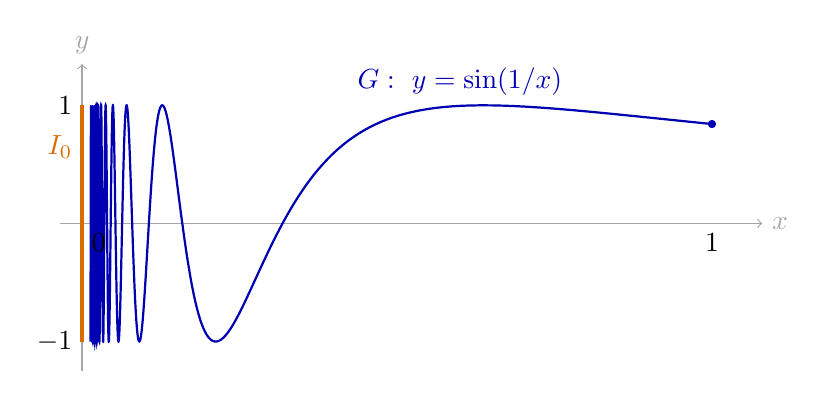
\begin{tikzpicture}[x=8cm,y=1.5cm]
	\draw[->,gray!70] (-0.035,0)--(1.08,0) node[right] {\(x\)};
	\draw[->,gray!70] (0,-1.25)--(0,1.35) node[above] {\(y\)};
	\draw[very thick,orange!85!black] (0,-1)--(0,1);
	\draw[blue!70!black,thick,domain=1:75,samples=1800,variable=\t] plot ({1/\t},{sin(\t r)});
	\fill[blue!70!black] (1,{sin(1 r)}) circle(1.5pt);
	\node[orange!85!black,left] at (0,0.65) {\(I_0\)};
	\node[blue!70!black] at (0.6,1.2) {\(G:\ y=\sin(1/x)\)};
	\node[below] at (1,0) {\(1\)};
	\node[left] at (0,-1) {\(-1\)};
	\node[left] at (0,1) {\(1\)};
	\node[below right] at (0,0) {\(0\)};
\end{tikzpicture}

	\caption[拓扑正弦曲线]{拓扑正弦曲线 \(S=G\cup I_0\)。曲线 \(G\) 不断靠近竖线段 \(I_0\)，使整个集合连通；沿一条道路离开竖线段却会迫使纵坐标在任意短的参数时间内反复走遍 \([-1,1]\)，与连续性矛盾。左侧密集振荡仅画出有限部分。}
	\label{g1:fig:topologist-sine}
\end{figure}

图中的竖线段不是与曲线“隔着一个正距离”的另一块：它的每个点都是曲线的极限点。这解释了为什么集合没有开集分离；道路的障碍则来自趋近竖线段时无限振荡的纵坐标。连通与道路连通分别检测了这两件不同的事。

\begin{definition}[局部道路连通]\label{g1:def:locally-path-connected}
	若拓扑空间 \(X\) 的每个点 \(x\)，在每个给定开邻域 \(U\) 中，都有一个道路连通开邻域 \(V\) 满足 \(x\in V\subseteq U\)，则称 \(X\)\term[jubudaoluliantong]{局部道路连通}[locally path-connected]。
\end{definition}

定义要求能够任意缩小，并非仅要求每点落在某个道路连通开集中。Euclid 开集局部道路连通，因为充分小的开球凸；局部同胚于 Euclid 开集的空间也局部道路连通，只需把小球送回原空间。拓扑正弦曲线在竖线段上的任何点都没有道路连通开邻域：每个这样的开邻域都遇到 \(G\)，而上一例已证明不存在从竖线段到 \(G\) 的道路。

\subsection{分支及其在映射下的行为}
\label{g1:subsec:0402:04}

一个空间未必整体连通，此时可以按“属于同一个连通部分”把点分组。这里的“部分”应是最大的连通子集，而不能只是任意选出的一个连通邻域；否则分组会依赖选择。

\begin{definition}[连通分支与道路分支]\label{g1:def:components}
	拓扑空间 \(X\) 的极大非空连通子集称为\term[liantongfenzhi]{连通分支}[connected component]。对 \(x\in X\)，所有可用道路从 \(x\) 到达的点组成的集合称为 \(x\) 的\term[daolufenzhi]{道路分支}[path component]。
\end{definition}

反向参数 \(t\mapsto1-t\) 可以反转道路；把两条道路分别重参数化到 \([0,1/2]\)、\([1/2,1]\) 并在公共端点相接，便可拼成一条道路。拼接的连续性由闭集粘合\cref{g1:prop:gluing-lemma}保证，因为两段在 \(t=1/2\) 取值相同。再加上常值道路，“可以用道路相连”就是等价关系。每个等价类本身道路连通：连接其中两点的道路经过的任一点，都能通过取道路的一段而与这两点相连，所以整条道路都留在同一个等价类中。因此道路分支也就是极大道路连通子集。

\begin{proposition}[分支的存在与基本性质]\label{g1:prop:components}
	设 \(X\) 为拓扑空间。
	\begin{enumerate}
		\item 对每个 \(x\in X\)，包含 \(x\) 的所有连通子集之并 \(C_x\) 是唯一包含 \(x\) 的连通分支；各连通分支构成 \(X\) 的一个划分。
		\item 每个连通分支闭于 \(X\)，但不一定开。每个道路分支包含在唯一的连通分支中。
		\item 若 \(f:X\to Y\) 连续，则一个连通分支的像包含在 \(Y\) 的某个连通分支中，一个道路分支的像包含在 \(Y\) 的某个道路分支中。
	\end{enumerate}
\end{proposition}
\begin{proof}
	第一项中，所有参加并集的连通子集都含 \(x\)，所以由\cref{g1:prop:connected-image-closure}，它们的并 \(C_x\) 连通。任何包含 \(x\) 的连通子集都已在此并中，因此 \(C_x\) 极大且唯一。如果两个这样的集合相交，它们的并仍连通，极大性便使两者相等；每个点至少属于自己的 \(C_x\)，所以这些分支构成划分。

	第二项中，\(\overline{C_x}\) 由同一命题仍连通，且包含 \(C_x\)，极大性给出 \(\overline{C_x}=C_x\)，故 \(C_x\) 闭。道路分支道路连通，因而连通，所以它包含在唯一的 \(C_x\) 中。连通分支未必开，例如 \(\mathbb Q\) 中每个连通分支都是单点，却没有单点是开集，证明见习题。

	第三项中，连通分支的连续像连通，因而被包含在其中任一点所属的连通分支中。对于道路分支，用道路与 \(f\) 复合即可说明其像道路连通，故同样被包含在某个道路分支中。
\end{proof}

此处结论是“包含在”，不能改成“等于”。例如常值映射把任意连通空间送到 \(\mathbb R\) 的一个点，而 \(\mathbb R\) 的连通分支是整个直线。甚至映射本身满射，也未必把每个分支满射到目标分支，习题将给出例子。

\begin{theorem}[局部道路连通时两种分支一致]\label{g1:thm:locally-path-components}
	若 \(X\) 局部道路连通，则 \(X\) 的每个道路分支都是开集，并且道路分支与连通分支相同。因此局部道路连通空间连通，当且仅当它道路连通。
\end{theorem}
\begin{proof}
	设 \(P\) 为一个道路分支，\(x\in P\)。局部道路连通性给出 \(x\) 的道路连通开邻域 \(V\)。\(V\) 中每点都能与 \(x\) 用道路连接，故 \(V\subseteq P\)。因此 \(P\) 中每点都有包含在 \(P\) 内的开邻域，\(P\) 开。

	设 \(C\) 为包含 \(P\) 的连通分支。若 \(C\setminus P\ne\varnothing\)，因为其他道路分支也开，\(X\setminus P\) 是开集；于是 \(P=C\cap P\) 与 \(C\setminus P=C\cap(X\setminus P)\) 是 \(C\) 的两个非空、不交相对开集，其并为 \(C\)，与 \(C\) 连通矛盾。因此 \(C=P\)。对非空连通空间，唯一的连通分支就是整个空间，所以结论随之成立；空空间也符合约定。
\end{proof}

拓扑正弦曲线说明局部条件的作用：它只有一个连通分支 \(S\)，却有两个道路分支 \(G,I_0\)，其中 \(I_0\) 不是开集。流形的局部 Euclid 性质则排除了这种现象。在流形上讨论某一连通分支时，也就在讨论一个开且道路连通的部分；这将允许我们把沿道路的局部构造在同一分支内传递。有关连通性、紧性和局部紧性的进一步阅读，可参阅\cite[第4章, Connectedness, 第86页; Compactness, 第94页; Local Compactness, 第104页]{Lee2011Topological}。
